\documentclass[letterpaper,10pt]{article}

\usepackage{enumitem}
\usepackage{titling}
\usepackage{listings,listings-rust}
\usepackage{url}
\usepackage{soul}
\usepackage{hyperref}
\usepackage{setspace}
\usepackage{subfig}
\usepackage{sectsty}
\usepackage{pdfpages}
\usepackage{colortbl}
\usepackage{multirow}
\usepackage{multicol}
\usepackage{relsize}
\usepackage{amsmath}
\usepackage{wasysym}
\usepackage{fancyvrb}
\usepackage[yyyymmdd]{datetime}
\usepackage{amsmath,amssymb,amsthm,graphicx,xspace}
\usepackage[titlenotnumbered,noend,noline]{algorithm2e}
\usepackage[compact]{titlesec}
\usepackage{XCharter}
\usepackage[T1]{fontenc}
\usepackage[scaled]{beramono}
\usepackage[normalem]{ulem}
\usepackage{booktabs}
\usepackage{tikz}
\usetikzlibrary{arrows.meta,automata,shapes,trees,matrix,chains,scopes,positioning,calc,decorations.pathreplacing}
\tikzstyle{block} = [rectangle, draw, fill=blue!20, 
    text width=2.5em, text centered, rounded corners, minimum height=2em]
\tikzstyle{bw} = [rectangle, draw, fill=blue!20, 
    text width=4em, text centered, rounded corners, minimum height=2em]

\definecolor{namerow}{cmyk}{.40,.40,.40,.40}
\definecolor{namecol}{cmyk}{.40,.40,.40,.40}
\renewcommand{\dateseparator}{-}

\let\LaTeXtitle\title
\renewcommand{\title}[1]{\LaTeXtitle{\textsf{#1}}}

\lstset{basicstyle=\footnotesize\ttfamily,breaklines=true}

\newcommand{\CPP}{C\nolinebreak\hspace{-.05em}\raisebox{.4ex}{\tiny\bf +}\nolinebreak\hspace{-.10em}\raisebox{.4ex}{\tiny\bf +}}
\def\CPP{{C\nolinebreak[4]\hspace{-.05em}\raisebox{.4ex}{\tiny\bf ++}}}

\newcommand{\handout}[5]{
  \noindent
  \begin{center}
  \framebox{
    \vbox{
      \hbox to 5.78in { {\bf ECE459: Programming for Performance } \hfill #2 }
      \vspace{4mm}
      \hbox to 5.78in { {\Large \hfill #4  \hfill} }
      \vspace{2mm}
      \hbox to 5.78in { {\em #3 \hfill \today} }
    }
  }
  \end{center}
  \vspace*{4mm}
}

\newcommand{\lecture}[3]{\handout{#1}{#2}{#3}{Lecture#1}}
\newcommand{\tuple}[1]{\ensuremath{\left\langle #1 \right\rangle}\xspace}

\addtolength{\oddsidemargin}{-1.000in}
\addtolength{\evensidemargin}{-0.500in}
\addtolength{\textwidth}{2.0in}
\addtolength{\topmargin}{-1.000in}
\addtolength{\textheight}{1.75in}
\addtolength{\parskip}{\baselineskip}
\setlength{\parindent}{0in}
\renewcommand{\baselinestretch}{1.5}
\newcommand{\term}{Winter 2020}

\singlespace


\begin{document}

\lecture{29 --- Clusters \& Cloud Computing}{\term}{Jeff Zarnett \& Patrick Lam}

\section*{Clusters and Cloud Computing}
Almost everything we've seen so far has improved performance on a single
computer. Sometimes, you need more performance than you can get on a
single computer, or you have reached a point where it's a lot better value for
your money to buy two cheap computers than one very expensive computer.
For the most part, if you could split your problem into
multiple threads or multiple processes, you can do the same with multiple
computers. We'll survey techniques for programming for
performance using multiple computers; although there's overlap with
distributed systems, we're looking more at calculations here.

\paragraph*{Message Passing.} Rust has encourages message-passing, but
a lot of your previous experience when working with C may have centred around
shared memory systems and you may have done that in Rust too (\texttt{Mutex}, 
anyone?). In some circumstances that we've seen, you don't have a choice!
The model of GPU programming meant we had to explicitly
manage copying of data. When we have multiple computers, shared memory is not
an option, so we have to use message passing. Fortunately, we know how to do
that. The only thing to note now is that communication over the network is
much more expensive than communicating within the same system, so we will
need to think carefully about how much to communicate.

There was a time when we would talk about MPI, the \emph{Message Passing 
Interface}, a de facto standard for programming message-passing multi-
computer systems. This is, unfortunately, no longer the way. 
MPI sounds good, but in practice people tend to use other things. 
Here's a detailed piece about the relevance of MPI today:~\cite{hpcmpi}, if 
you are curious. 

\paragraph{REST}
We've already seen asynchronous I/O using HTTP (curl) which we could use to
consume a REST API as one mechanism for multi-computer communication. You
may have also learned about sockets and know how to use those, which would
underly a lot of the mechanisms we're discussing. The socket approach is too
low-level for what we want to discuss, and while the REST API approach is at a
reasonable level of abstraction. 

REST APIs are often completely synchronous, but don't have to be: 
you can set up  callbacks to be notified when a computation is done, or
the caller can check back later to see if the request is finished. But these
aren't truly asynchronous, because the remote machine has to be available at
the time of each call. Perhaps we'd like to decouple services even more than
that and use something else...

\paragraph{Kafka.} 
Let's talk about Apache Kafka, a self-described ``distributed streaming platform'' that's got significant adoption in industry as a mechanism of communication between different services running over a network. For a breakdown on how it works, we're using~\cite{kafka} as a guide.

Communication is based around the idea of producers writing a record (some data element, like an invoice) into a topic (categorizing messages) and consumers taking the item from the topic and doing something useful with it. A message remains available for a fixed period of time and can be replayed if needed. I think at this point you have enough familiarity with the concept of the producer-consumer problem and channels/topics/subscriptions that we don't need to spend a lot of time on it. 


Kafka's basic strategy is to write things into an immutable log. The log is split into different partitions; you choose how many when creating the topic, where more partitions equals higher parallelism. The producer writes something and it goes into one of the partitions. Consumers read from each one of the partitions and writes down its progress (``commit its offset'') to keep track of how much of the topic it has consumed.  See this image from \url{kafka.apache.org}:

\begin{center}
	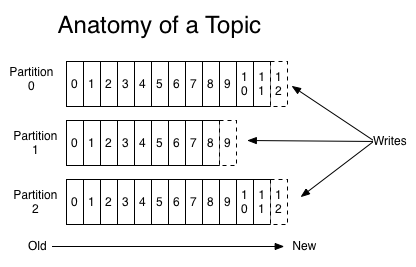
\includegraphics[width=0.4\textwidth]{images/kafka-partition.png}
\end{center}

The nice part about such an architecture is that we can provision the parallelism that we want, and the logic for the broker (the system between the producer and the consumer, that is, Kafka) is simple. Also, consumers can take items and deal with them at their own speed and there's no need for consumers to coordinate; they manage their own offsets. Messages are removed from the topic based on their expiry, so it's not important for consumers to get them out of the queue as quickly as possible.

Quick aside on that: under normal circumstances, in something like a standard queue, there's a little bit of pressure to get items out of the queue quickly. If the queue is growing, it might mean the queue is full and new items can't be produced or are thrown away... or perhaps you get charged money for the storage space the queue is using. 

You might think that it's a solution to take the item out of the queue in one transaction and then process it later. That's okay only if you've successfully saved it to a database or other persistent storage. Otherwise, you could take the item out and a crash or called shutdown means that the item doesn't actually get processed. Oops!

\paragraph{Alternatives.} There's also some popular AWS (Amazon Web Services)-based solutions for this kind of multiple computer communication: SNS (Simple Notification Service) and SQS (Simple Queueing Service). They are, broadly speaking, just other ways to decouple the communication of your programs.

SNS is good for sending lots of messages to multiple receivers, maybe push notifications or making sure all systems update their records or that you send pager alerts to people about things that have gone wrong. SNS messages are not persistent, so if you miss it, you miss it. 

SQS is more for batches of work where it's not particularly time-sensitive and the item will be consumed by a worker. SQS data is deleted after being taken out of the queue and may or may not have ordering guarantees. SQS does have limits on how long a message can be stored, though. 

\subsection*{Cloud Computing}
We'll start with a little bit of history.
In the old days, if you wanted a cluster, you had to find a bunch of
money to buy and maintain a pile of expensive machines. Not anymore.
Cloud computing is perhaps way overhyped, but we can talk about 
one particular aspect of it, as exemplified by Amazon's Elastic
Compute Cloud (EC2).

Consider the following evolution:
\begin{itemize}
\item Once upon a time, if you wanted a dedicated server on the
  Internet, you had to get a physical machine hosted, usually in a
  rack somewhere. Or you could live with inferior shared hosting.
\item Virtualization meant that you could instead pay for part of a
  machine on that rack, e.g. as provided by {\tt slicehost.com}.  This
  is a win because you're usually not maxing out a computer, and you'd
  be perfectly happy to share it with others, as long as there are
  good security guarantees. All of the users can get root access.
\item Clouds enable you to add more machines on-demand. Instead of
  having just one virtual server, you can spin up dozens (or
  thousands) of server images when you need more compute
  capacity. These servers typically share persistent storage, also in
  the cloud. 
\end{itemize}

In cloud computing, you pay according to the number of machines, or
instances, that you've started up. Providers offer different instance
sizes, where the sizes vary according to the number of cores, local
storage, and memory. Some instances even have GPUs, but it seemed 
uneconomic to use this for Assignment 3, at least in previous years (I
have not done the calculation this year). 
Instead we have the {\tt ecetesla} machines.

\paragraph{Launching Instances.} When you need more compute power,
you launch an instance. The input is a virtual machine image.  You use
a command-line or web-based tool to launch the instance.  After you've
launched the instance, it gets an IP address and is
network-accessible. You have full root access to that instance.

Amazon provides public images which run a variety of operating
systems, including different Linux distributions, Windows Server, and
OpenSolaris. You can build an image which contains the software you
want, including Hadoop and OpenMPI.

\paragraph{Terminating Instances.} A key part of cloud computing is
that, once you no longer need an instance, you can just shut it down
and stop paying for it. All of the data on that instance goes away.

\paragraph{Continuous Deployment.} The combination of launching and terminating instances can mean that updates don't require downtime: you start up the new instances and then shut down the old ones so there's no gap where the service is down.

Sometimes this causes slight headaches, like if you make a database change that's incompatible: the old nodes will have a problem, so you need to be a little careful with this.

\paragraph{Storing Data.} You probably want to keep some persistent results
from your instances. Basically, you can either mount a storage device,
also on the cloud (e.g. Amazon Elastic Block Storage); or, you can
connect to a database on a persistent server (e.g. Amazon SimpleDB or
Relational Database Service); or, you can store files on the Web
(e.g. Amazon S3). 


\section*{Clusters versus Laptops}
There is a paper about this: Frank McSherry, Michael Isard, Derek G. Murray. ``Scalability! But at what COST?'' HotOS XV. This part of the lecture is based on the companion blog post~\cite{scalecost}.

The key idea: scaling to big data systems introduces substantial overhead. Let's just see how, say, a laptop compares, in absolute times, to 128-core big data systems.

\paragraph{Summary.} Big data systems haven't yet been shown to be obviously good; current evaluation is lacking.
The important metric is not just scalability; absolute
performance matters a lot too. We don't want a situation where we are just scaling up to $n$ systems to deal with the complexity of scaling up to $n$ systems. Or, as Oscar Wilde put it: ``The bureaucracy is expanding to meet the needs of the expanding bureaucracy.''

\paragraph{Methodology.} We'll compare a competent single-threaded implementation to top
big data systems, as described in an OSDI 2014 (top OS conference) paper on GraphX\cite{graphx}. The domain: graph processing
algorithms, namely PageRank and graph connectivity (for which the bottleneck is label propagation). The subjects: graphs with billions of edges, amounting to a few
GB of data.

\paragraph{Results.} 128 cores don't consistently beat a laptop at PageRank: e.g. 249--857s on the twitter\_rv dataset for the big data system vs 300s for the laptop, and they are 2$\times$ slower for label
propagation, at 251--1784s for the big data system vs 153s on
twitter\_rv. From the blogpost:

\begin{center}
	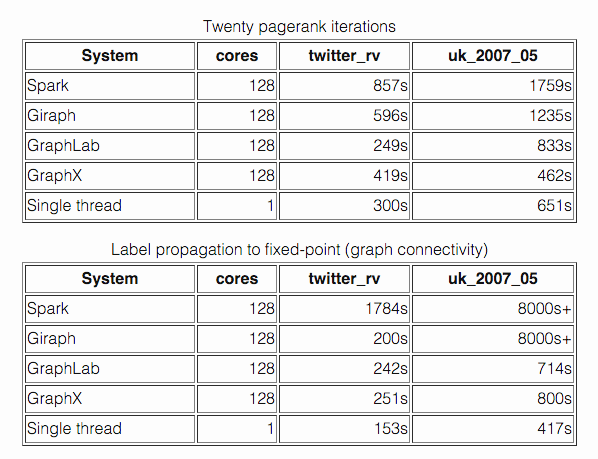
\includegraphics[width=0.60\textwidth]{images/pagerank.png}
\end{center}

\paragraph{Wait, there's more.} I keep on saying that we can improve algorithms for additional performance boosts too.
But that doesn't generalize, so it's hard to teach. In this case, two improvements are: using Hilbert curves
for data layout, improving memory locality, which helps a lot for PageRank; and using a union-find algorithm 
(which is also parallelizable). ``10$\times$ faster, 100$\times$ less embarrassing''.  We observe an overall
$2\times$ speedup for PageRank and $10\times$ speedup for label propagation.

\paragraph{Takeaways.} Some thoughts to keep in mind, from the authors:
\begin{itemize}
\item    ``If you are going to use a big data system for yourself, see if it is faster than your laptop.''
\item    ``If you are going to build a big data system for others, see that it is faster than my laptop.''
\end{itemize}



\section*{Movie Hour}
Let's take a humorous look at cloud computing: James Mickens' session from Monitorama PDX 2014. 

\begin{center}
\url{https://vimeo.com/95066828}
\end{center}

\bibliographystyle{alphaurl}
\bibliography{459}


\end{document}
